%
% File coling2020.tex
%
%% Based on the style files for COLING-2018
%

\documentclass[11pt]{article}
\usepackage{coling2020}
\usepackage{times}
\usepackage{url}
\usepackage{latexsym}

\setlength\titlebox{4cm}
\colingfinalcopy

\title{ML Model Analysis}

\author{
      \\
    An analysis of machine learning models and their applications. \\
    by Kai Hulme \\ 
    % University of Bristol \\
    % 26th July 2021 \\
}

\begin{document}

\maketitle
\newpage

%%%%%%%%%%%%%%%%%%%%%%%%%%%%%%%%%%%%%%%%%%%%%%%%%%%%%%%%%%%%%%%%%%%%%%%%%%%%%%%%%%%%%%%%%%%%%%%%%%%%%%%%
%%%%%%%%%%%%%%%%%%%%%%%%%%%%%%%%%%%%%%%%%%%%%%%%%%%%%%%%%%%%%%%%%%%%%%%%%%%%%%%%%%%%%%%%%%%%%%%%%%%%%%%%
%%%%%%%%%%%%%%%%%%%%%%%%%%%%%%%%%%%%%%%%%%%%%%%%%%%%%%%%%%%%%%%%%%%%%%%%%%%%%%%%%%%%%%%%%%%%%%%%%%%%%%%%

\section{Unsupervised Learning}
\label{analysing_mnist}

\subsubsection{Unsupervised learning}

Unsupervised learning does not require a target label to learn from the data. Without guidance from a target label an unsupervised method cannot predict or classify, instead it aims to represent the data in some way. This could be clustering data into distinct groups, representing the data as a reduced set of its features or detect anomalous entries in a dataset. 

\subsubsection{MNIST}

The MNIST dataset is a collection of 70000 28x28 grey scale images of handwritten digits (0-9). The dataset is comprised of 784 features describing the individual pixel intensity (0-255) for each image, along with an additional target feature describing the digit the image represents.

\subsubsection{The curse of dimensionality}

Having a lot of features can accurately describe the nature of the real data, but additional features comes additional complexity. In high dimensional space it can be hard for models to accurately represent the data as each point becomes further away to the point where with enough features each entry can seem equidistant - this is often an issue when there are more entries than features; the curse of dimensionality refers to this trade off.

\subsubsection{Dimensionality reduction}

The aim of dimensionality reduction is the reduce the number of features in a dataset whilst retaining what makes the data unique. It is common place in exploratory data analysis to get an understanding of the distribution of importance across the features. The higher dimension dataset is mapped into a lower dimensional space whilst retaining the maximum amount of variance.

%%%%%%%%%%%%%%%%%%%%%%%%%%%%%%%%%%%%%%%%%%%%%%%%%%%%%%%%%%%%%%%%%%%%%%%%%%%%%%%%%%%%%%%%%%%%%%%%%%%%%%%%

\subsection{Principal Component Analysis}
\label{pca}

Principle component analysis is a projection method of dimensionality reduction. PCA produces a set of component vectors where the first explains the most variance in the data and the next vector is orthogonal to that and explains the next most and so on.

\subsubsection{Applying PCA to MNIST}

Figure \ref{pca_variance} shows a plot of cumulative variance contribution for each principal component from most to least variance, along with reconstructions of sample images from decreasing levels of dimensionality reduction. These results show that 90\% of the variance in the MNIST dataset can be explained by approximately 75 principal components. \\

The reconstructions show recognisable images for 100 and 25 components. With 5 of the components, the reconstructions are recognisable as digits, but class independence is lost. This indicates most of the image can be represented by few features, which is unsurprising given most of the images consist of black backgrounds with white areas of similar size and shape.

\begin{figure}[h]
    \centering
    \begin{minipage}{0.45\textwidth}
        \centering
        \fbox{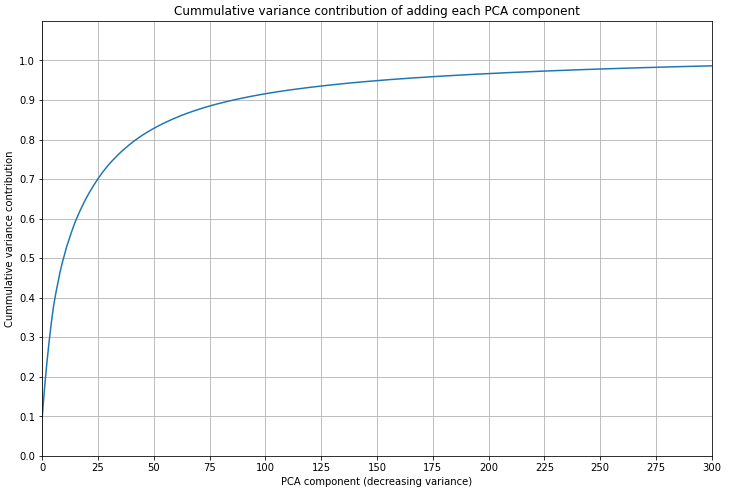
\includegraphics[height=0.7\linewidth]{figures/01_analysing_mnist/pca_cummulative_variance.png}}
    \end{minipage}\hfill
    \begin{minipage}{0.45\textwidth}
        \centering
        \fbox{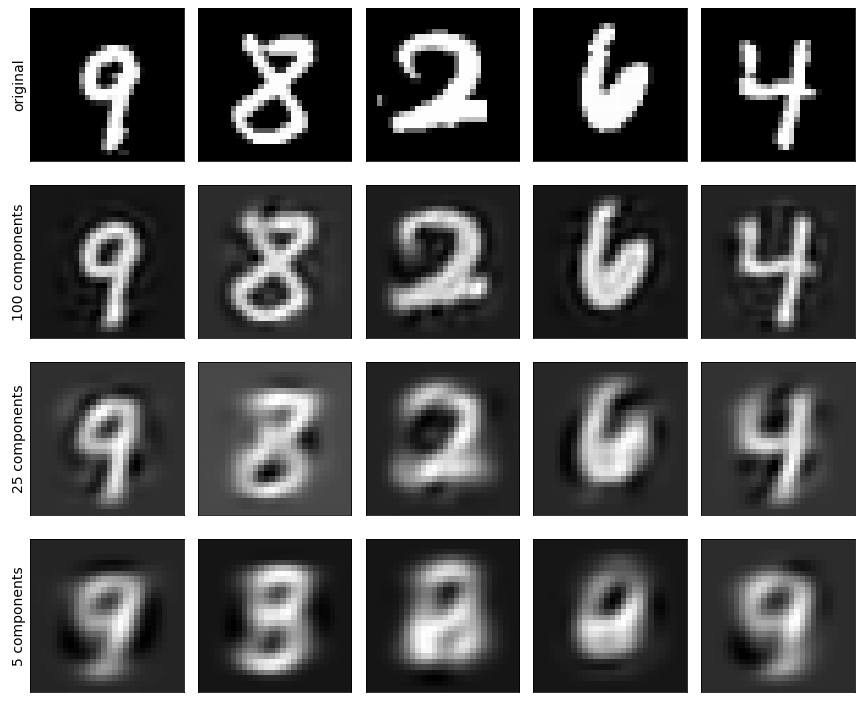
\includegraphics[height=0.7\linewidth]{figures/01_analysing_mnist/pca_component_reconstructions.png}}
    \end{minipage}
    \caption{Cumulative variance contribution for increasing PCA components of MNIST dataset (left) and reconstructions of sample images from decreasing number of components (right).}
    \label{pca_variance}
\end{figure}

\subsubsection{Dimensionality Reduction for Visualisation}

It's difficult to view information which has more than 3 dimensions. For this reason, it's often a good idea to use dimensionality reduction to reduce the number of dimensions, allowing us to visualise the data in a way we can understand. Figure \ref{mnistvis} shows a visualisation of the MNIST dataset reduced to 2 dimensions. Each colour represents a class. There are clear groupings of classes, but there are limited separations between them, making it difficult to identify clusters. T-distributed Stochastic Neighbour Embedding (t-SNE) is another dimensionality reduction method, which often works better for visualisation than PCA. t-SNE aims to keep similar classes together and other further apart. This results in  clearer class separation, shown in Figure \ref{mnistvis}.

\begin{figure}[h]
    \centering
    \begin{minipage}{0.45\textwidth}
        \centering
        \fbox{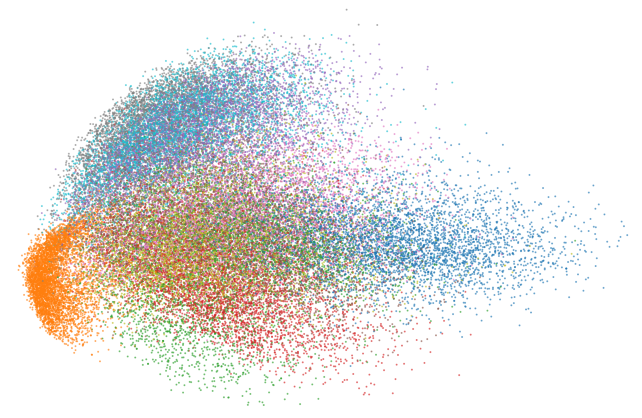
\includegraphics[height=0.6\linewidth]{figures/01_analysing_mnist/mnist_pca_2d.png}}
    \end{minipage}\hfill
    \begin{minipage}{0.45\textwidth}
        \centering
        \fbox{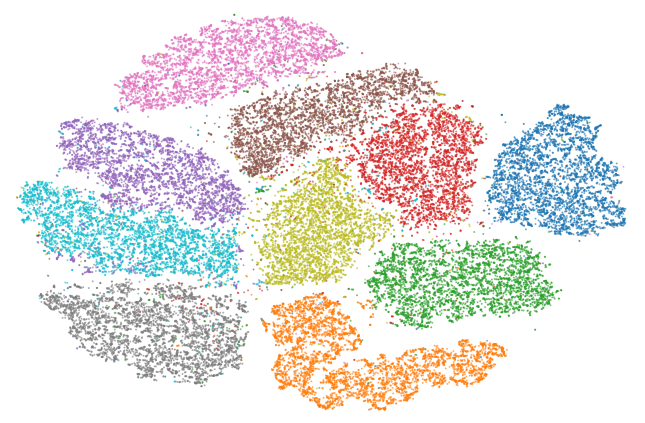
\includegraphics[height=0.6\linewidth]{figures/01_analysing_mnist/mnist_tsne_2d.png}}
    \end{minipage}
    \caption{Visualisation of MNIST reduced to 2 dimensions by PCA (left) and t-SNE (right).}
    \label{mnistvis}
\end{figure}

%%%%%%%%%%%%%%%%%%%%%%%%%%%%%%%%%%%%%%%%%%%%%%%%%%%%%%%%%%%%%%%%%%%%%%%%%%%%%%%%%%%%%%%%%%%%%%%%%%%%%%%%

\subsection{Clustering}
\label{kmeans}

\subsubsection{K-Means}

K-Means is a clustering method, which is used to cluster the dataset into K-clusters. The centre of each cluster is defined by a centroid, whose position which is the mean of each data point assigned to that cluster. K-Means can be used to group similar data points together without the need for class labels.

\subsubsection{Clustering MNIST}

\begin{figure}[h]
\floatbox[{\capbeside\thisfloatsetup{capbesideposition={right,top},capbesidewidth=9cm}}]{figure}[\FBwidth]
{\caption{Voronoi diagram from K-Means clustering of MNIST dataset reduced to 2 dimensions by PCA with coloured cluster boundaries and centroids marked with $X$, with sample of reduced data plotted with $\alpha=0.1$ (denser areas of points appear darker). The group of orange points in the lower left part of Figure 2 appear clustered into the light blue cluster represented in Figure 3. There are similar similarities between other groups of points and the clusters, but is mostly inaccurate as there's not much separation between the classes in the PCA - clustering on the t-SNE reduction may look better.}}
{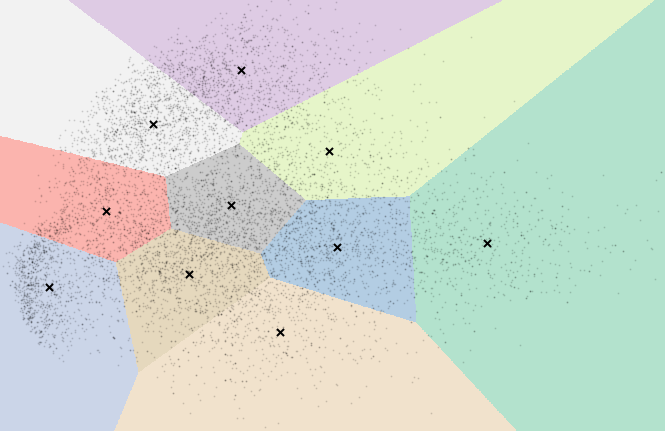
\includegraphics[height=0.65\linewidth]{figures/01_analysing_mnist/kmeans_voronoi.png}}
\label{voroni}
\end{figure}

% \begin{figure}[h]
%     \centering
%     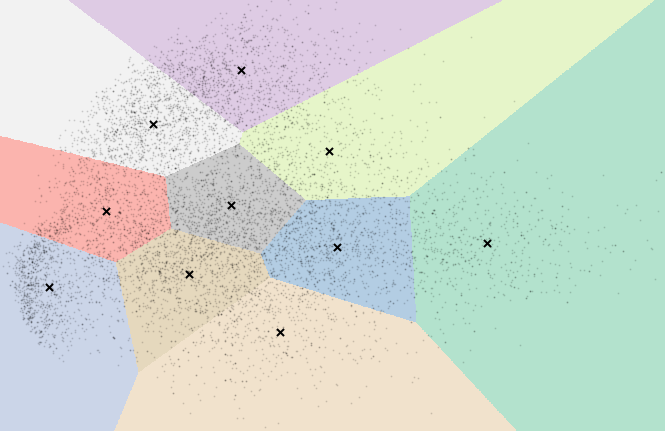
\includegraphics[height=0.3\linewidth]{figures/01_analysing_mnist/kmeans_voronoi.png}
%     \caption{Voronoi diagram from K-Means clustering of MNIST dataset reduced to 2 dimensions by PCA with coloured cluster boundaries and centroids marked with $X$, with sample of reduced data plotted with $\alpha=0.1$ (denser areas of points appear darker).}
% \end{figure}

\subsubsection{K-Means Performance}

Measuring K-Means performance can be difficult. Firstly data points can seem equidistant in a high enough dimension space, but also as K-Means is an unsupervised method it does not learn class labels so its labelling is arbitrary and doesn't align with the real labels so it can be difficult to assess cluster accuracy but there are some useful metrics specific to K-Means. Silhouette score is a measure of the distance between points and the closest cluster (like inertia) but scaled in a way which results in a score of 1 being the optimal clustering solution and numbers above 0 being good clustering solutions. Negative numbers indicate poor clustering performance or non-convergence. Adjusted random score attempts to measure similarity between the real labels and the K-Means cluster labels allowing for accuracy to be calculated despite random cluster labels.Here we have a score of , which is good considering how mixed the classes are in 2 dimensions. Clustering on the reduced MNIST dataset achieves a silhouette score of $0.36$ and adjusted random score of $0.29$, which is good given the inter-class mixing in the 2D projection.

\newpage

%%%%%%%%%%%%%%%%%%%%%%%%%%%%%%%%%%%%%%%%%%%%%%%%%%%%%%%%%%%%%%%%%%%%%%%%%%%%%%%%%%%%%%%%%%%%%%%%%%%%%%%%
%%%%%%%%%%%%%%%%%%%%%%%%%%%%%%%%%%%%%%%%%%%%%%%%%%%%%%%%%%%%%%%%%%%%%%%%%%%%%%%%%%%%%%%%%%%%%%%%%%%%%%%%
%%%%%%%%%%%%%%%%%%%%%%%%%%%%%%%%%%%%%%%%%%%%%%%%%%%%%%%%%%%%%%%%%%%%%%%%%%%%%%%%%%%%%%%%%%%%%%%%%%%%%%%%

\section{Classification}
\label{classifiers}

\subsubsection{Supervised learning and classification}
\label{supervised_learning}

In supervised machine learning each sample in the training data has a label which describes the data in some desirable way, called the \textit{target label}. This target label is used to teach the model what it is about the data that you want to learn. Classification models aim to predict the target label (classify) of a given entry.

\subsubsection{Overfitting and underfitting}

A model with enough parameters can trivially learn how to explain a dataset it was trained with by the samples given target labels, but this is not the aim of machine learning. A good machine learning model will be able to make accurate predictions of unseen data from distributions learnt in unseen data which are present in the unseen data. A model which performs well making predictions from training data but poorly when predicting unseen data is a model which has overfit; a model which does not overfit is one which generalises to unseen data well. When a model is unable to make accurate predictions of the training data it has underfit - this may be because the model has not seen enough training data, is poorly optimised or lacks enough parameters to represent the data in the desired way.

\subsubsection{Cross-Validation}
\label{crossval}

When creating a validation set to validate a model during training there is an element of bias in how the validation data was taken from the overall dataset. Cross-validation helps to mitigate lucky sampling by training on all of the training data by splitting the training data into $K$ groups (folds). The model is trained $K$ times, each time using a different fold for validation and the remaining folds for model training. You can then observe the mean performance to get an accurate indication of (average) real world performance, as well as the standard deviation. A good model will have low variance between folds indicating good performance is not a result of lucky sampling.

\subsubsection{No Free Lunch}

When model performance is averaged across all possible problems, all models will perform the same, or no better than random - there is no free lunch. The insight here is that every model has bias, working on assumptions and chance. Model performance depends on the problem structure it faces.

%%%%%%%%%%%%%%%%%%%%%%%%%%%%%%%%%%%%%%%%%%%%%%%%%%%%%%%%%%%%%%%%%%%%%%%%%%%%%%%%%%%%%%%%%%%%%%%%%%%%%%%%

\subsection{Neural Networks}
\label{anns}

\subsubsection{Neurons, layers and activation functions}

ANNs are a network of neurons, similar to those in our brain, having a number of input signals each with a weighting (and a bias). The input signals are weighted and biased and their output is the result of a function called the activation function. This works similarly to the thresholding in a biological neurons soma, but the computation can take many forms. Neurons are organised in layers; many neurons in a layer, and many layers of neurons working together in the network. The input (layer) to the network is has $N$ neurons, where $N$ is the number of input features. There are then a additional (hidden) layers which perform computation on their inputs, passing their outputs to the next layer. The final (output) layer gives the resulting computation from the network. The following equation computes the outputs of each node in a layer from the inputs of the previous layer:

\[ h_{W,b}(X)=\phi(XW+b) \]

\begin{itemize}
\setlength\itemsep{0em}
\item $\phi$: the activation function applied to the weighted and biased inputs.
\item $X$: the matrix of input features from the previous layer.
\item $W$: the matrix of weights between the input and receiving neurons.
\item $b$: the bias vector, containing the bias term for each neuron.
\end{itemize}

The softmax activation function $(1)$ is used as the output activation function for a multi-classification, outputting probabilities (0 to 1) for each class. The rectified linear unit (ReLU) activation function $(2)$ is simpler than the softmax function; it is simply the maximum of the input or 0. Its simplicity means it is fast to compute and is the default choice for activation functions of hidden layers in many ANNs. \\

\begin{minipage}{.4\linewidth}
\begin{equation}
\centering
softmax(y)_i=\frac{e^{y_i}}{\sum_{j=1}^{n}{e^{y_j}}}
\end{equation}
\end{minipage} 
\begin{minipage}{.4\linewidth}
\begin{equation}
ReLU(x)=max(0,x)
\end{equation}
\end{minipage}

\subsubsection{Training neural networks}

Feed-forward ANNs are trained in two key stages, forward propagation where an input is fed through the network and a loss metric is calculated and back-propagation where a loss-optimiser is used to minimise the loss throughout the network. Back-propagation works by calculating the gradient of the loss function with respect to each weight using the chain rule one layer at a time, going backwards through the network from the output layer. \\

Stochastic gradient descent (SGD) is a common optimiser which allows for fast loss optimisation by estimating a subset of loss gradients rather than finding true derivatives. As the solution space of loss optimisation in ANNs is highly complex this estimation is needed for reasonable training times. The learning rate of an optimiser decides the rate at which it will head towards a better solution - higher learning rates will move faster through the solution space, but may take steps which are too big and miss good solutions.

\subsubsection{ANN Classification of MNIST}

To perform classification of the MNIST dataset I first normalised the pixel values so they were bound between 0 and 1 as this tends to work better with the smaller weight and bias values. I then created a training set to train the network, a validation set to monitor performance during training and a hold-out test set to test the models performance on unseen data. \\

Using an ANN of three dense (fully-connected) layers of 64 nodes with ReLU activation functions, followed by an output softmax layer of 10 nodes (one for each class) and optimised with SGD with categorical cross-entropy loss, my initial model achieved an test accuracy of $0.96$ in only 10 training epochs. The models training accuracy was $0.97$ which suggests some overfitting could be occurring.

\subsubsection{Learning rate optimisation}

\begin{figure}[h]
\floatbox[{\capbeside\thisfloatsetup{capbesideposition={right,top},capbesidewidth=9cm}}]{figure}[\FBwidth]
{\caption{This graph shoes the categorical cross-entropy (loss) of 5 ANNs (green, orange, red, pink, grey) with learning rates of 1, 0.1, 0.01, 0.001 and 0.0001 over 10 training epochs. The green model has a learning rate which is too high and is unable to learn from the dataset. The other models from orange to grey have increasing learning rates and this is reflected by the rate at which loss decreases throughout the epochs. \\ \\ A learning rates of 0.001 would be good choices as it converges on a solutions quickly with less risk of missing good solutions than higher rates. Another option would be to use learning rate scheduling to decrease rate throughout training, whether it be at each epoch or whenever there is a plateau in training progression.}}
{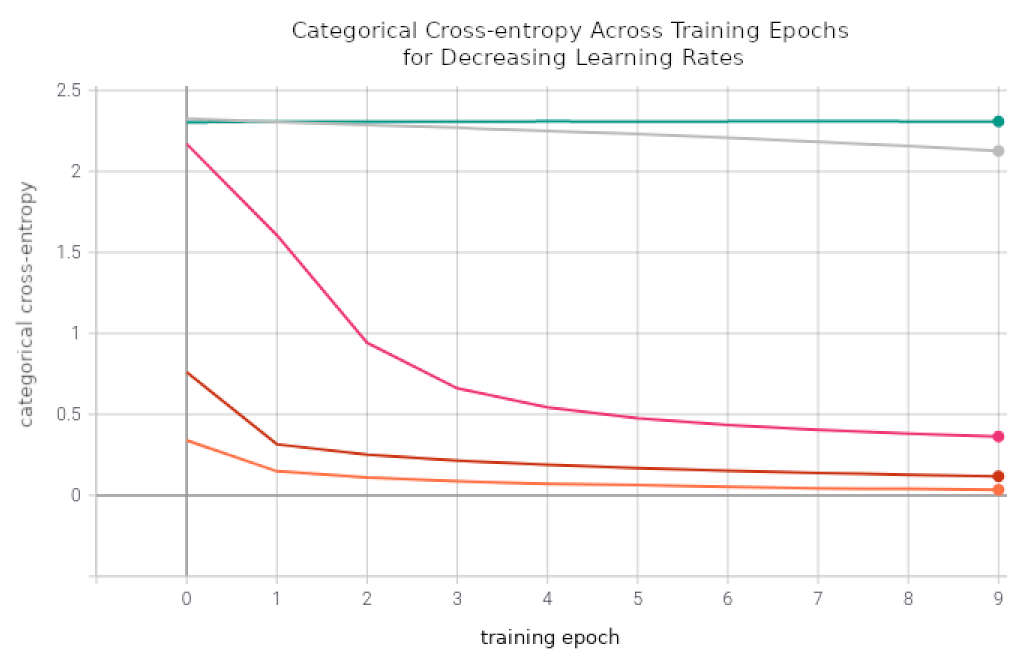
\includegraphics[height=0.65\linewidth]{figures/02_classification/learning_rates.png}}
\label{learning_rates}
\end{figure}

\subsubsection{Overfitting in neural networks}

Large ANNs can have millions of trainable parameters which can lead to models overfitting. There are a number of optimisations which I made to help with this. The first was to stop training once the validation loss plateaued (early stopping). Next was to train the model in batches of 32 samples and perform batch normalisation to normalise layer outputs which can increase training stability and convergence rate. I also added a 50\% dropout to a later layer of the network which ignores 50\% of the neurons in a layer - the idea being that the network learns to not rely too much on certain neurons which improves generalisation. I also used the Adam optimiser to dynamically change the momentum during training, which is used to accelerate training in areas with steeper gradients usually resulting in faster convergence. After these optimisations were applied the model achieved a testing accuracy of $0.97$.

\subsubsection{Convolutional neural networks}

Convolutional neural networks (CNNs) make use of convolutional kernels to create feature maps which when layered together can learn complex patterns in images. I created a CNN model which reshaped the input of the network to (28x28) images before 2 convolutional layers with 32 filters of (3x3) kernels followed by applying batch normalisation. The feature map outputs were then flattened and fed through two dense layers with a 50\% dropout rate between them, finally outputting class predicted probabilities. The resulting network when trained with the Adam optimiser (with a learning rate which decreases on validation loss plateau) until training progress stopped (at 31 epochs) gave an accuracy of $0.99$ on the hold-out test set.

\subsection{Support Vector Machines}
\label{svms}

Support vector machines (SVMs) are a family of machine learning models which aim to classify points in high dimensional space by finding the hyperplane that best separates the samples. It does so on a class-by-class basis and so for multi-class classification SVMs are trained for each class and used in a 1 vs. many fashion. 
\subsubsection{Soft-Margin}

Data is not always completely separable by a hyperplane. Soft-margin classification allows for a number of data points to be miss-classified which can allow erroneous data points to be ignored giving a better separating hyperplane. However, too soft of a margin and the hyperplane may not be the best fit. Sklearn allows for soft-margin SVM classification by altering the $c$ parameter. With a linear SVM classifier I used 3-fold cross-validation in a parameter grid search and found a soft margin $1\%$ the size of the training set to give optimal accuracy of $0.90$.

\subsubsection{Kernel SVMs}

Linear SVMs can perform well but require linear separation of classes. It is possible to apply a function (or kernel) to the data to allow for non-linear hyperplanes. Kernel SVMs make use of the kernel trick to function on the dataset as if it had been transformed without having to compute the (sometimes complex) transformation beforehand. This can result in fast non-linear classification with high accuracy. \\

I performed a grid search to optimise hyperparameters with 3-fold cross-validation on SVMs with linear, polynomial, radial basis function (RBF) and sigmoid kernels. The results showed the RBF kernel performed best with an accuracy of $0.975$, followed by the polynomial kernel of degree 2, the linear SVM and then sigmoid kernel with accuracies of $0.971$, $0.931$ and $0.924$ respectively. The RBF kernel often works well in most cases and has performed best and so I shall be using it for further comparisons to the SVM classification method.

\subsection{Comparison of Methods}

Both ANNs and SVMs are capable of non-linear classification of data thanks to non-linear activation functions of ANNs and kernel tricks of SVMs. The non-linear decision boundaries can be seen in \ref{decision_boundaries} for classification performed on the PCA reduced 2D MNIST dataset. SVMs usually do not require as much data as neural networks, e.g. a scenario with 2 samples is easily separable by a SVM, but a neural network will need more samples to generalise. For this reason it is best to use SVMs on smaller datasets and neural networks on larger (big) datasets. For the MNIST data set, as shown by strong performance across all models, either will work. CNNs have a slight edge, but for more complex (vision) tasks this advantage will grow.

\begin{figure}[h]
    \centering
    \begin{minipage}{0.45\textwidth}
        \centering
        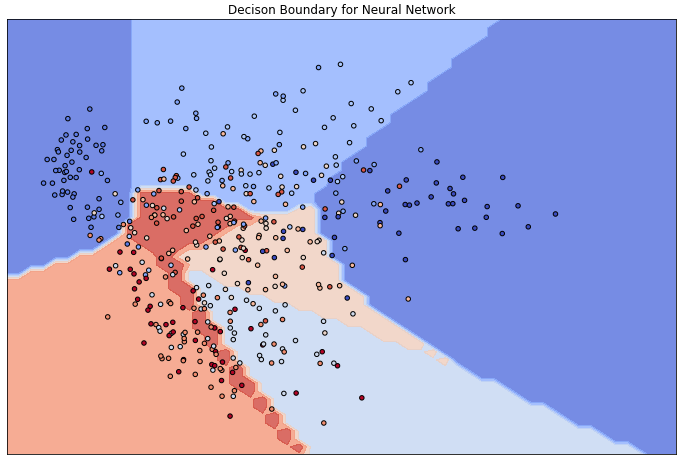
\includegraphics[height=0.6\linewidth]{figures/02_classification/nn_decision_boundary.png}
    \end{minipage}\hfill
    \begin{minipage}{0.45\textwidth}
        \centering
        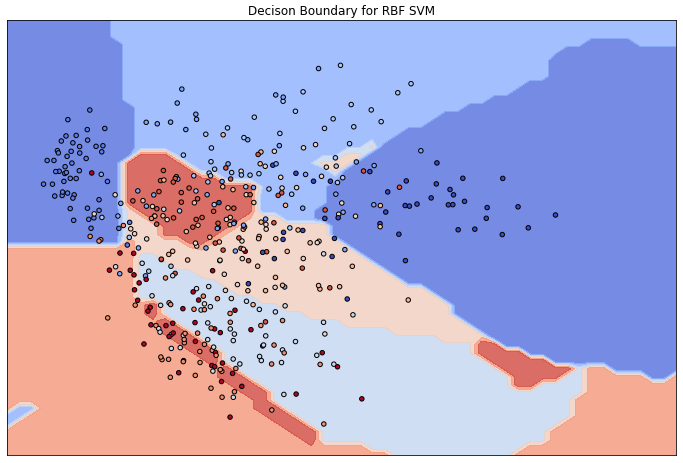
\includegraphics[height=0.6\linewidth]{figures/02_classification/svm_decision_boundary.png}
    \end{minipage}
    \caption{Decision boundary for neural network (left) and RBF-SVM (right) classification of MNIST reduced to 2 dimensions with PCA. Both are highly non-linear, but the decision boundaries of the neural network are a little clearer, although interpretability is difficult due to poor classification performance on the MNIST dataset when trained on only 2 PCA components.}
    \label{decision_boundaries}
\end{figure}

\newpage

%%%%%%%%%%%%%%%%%%%%%%%%%%%%%%%%%%%%%%%%%%%%%%%%%%%%%%%%%%%%%%%%%%%%%%%%%%%%%%%%%%%%%%%%%%%%%%%%%%%%%%%%
%%%%%%%%%%%%%%%%%%%%%%%%%%%%%%%%%%%%%%%%%%%%%%%%%%%%%%%%%%%%%%%%%%%%%%%%%%%%%%%%%%%%%%%%%%%%%%%%%%%%%%%%
%%%%%%%%%%%%%%%%%%%%%%%%%%%%%%%%%%%%%%%%%%%%%%%%%%%%%%%%%%%%%%%%%%%%%%%%%%%%%%%%%%%%%%%%%%%%%%%%%%%%%%%%

\section{Bayesian Linear Regression}
\label{bayesian_linear_regression}

\subsubsection{Bayesian Statistics and Regression}

Bayesian statistics is an approach to computing probabilities based on the belief that we can use prior knowledge of a domain to give better results. A Bayesian approach can be taken with linear regression; in a frequentist approach a model is fit to data to predict a target variable from a number of independent variables - the regression model aims to find the coefficients for these independent variables, in Bayesian regression prior knowledge is embedded into the model and the result is a distribution of variable coefficients, rather than an exact values.

\subsubsection{California Housing Dataset}

The California housing dataset consists of housing data information for blocks in California with features such as median house price, geographical location and number of rooms. The aim of regression on this dataset is to predict the median house price of a block given the independent features. \\

Plot $a$ below shows geographical data, with red areas indicating high median house price with larger dots indicating higher population. It is clear to see a housing price is clustered around a few key points; checking the longitude and latitude values in the dataset I found that they relate to real locations in California and concluded that the red areas were LA and San Francisco and where the points stop are the coast (lower-left) and the Californian border (upper-right). To encode this knowledge into the dataset I found the coordinates of the 10 most expensive areas to live in California and created a new feature to encode the distance to the nearest expensive area. This resulted in a new feature which had the second highest Pearson's correlation with the median house value after median income. \\

Further analysis of the features led me to the following pre-processing steps:

\begin{itemize}
    \setlength\itemsep{0em}
    \item Creation of new features representing bedrooms per room, bedrooms per occupant, number of additional rooms and estimated number of houses in the block.
    \item Removal of entries thresholded entries resulting in over-representation of single values in the distribution.
    \item Taking log of log-normal features so they fit a normal distribution.
    \item Centering of data around 0 mean and scaling to have unit variance.
    \item Perform a quantile transform to better fit normally distributed features to the normal distribution.
    \item Reduction of feature set to most correlating features: income, occupancy, house value, bedrooms per room, number of additional rooms, estimated number of houses in block and distance to the nearest expensive town. 
\end{itemize}

Plot $b$ shows a pair-plot showing pairwise scatter plots for each variable respective histograms on the diagonal after all pre-processing has been applied. It is clear that the variables now all fit a normal distribution and we can model it as such, using the normal distribution as the prior for Bayesian regression.

\begin{figure}[h]
    \label{california_eda}
    \centering
    \begin{minipage}{0.45\textwidth}
        \centering
        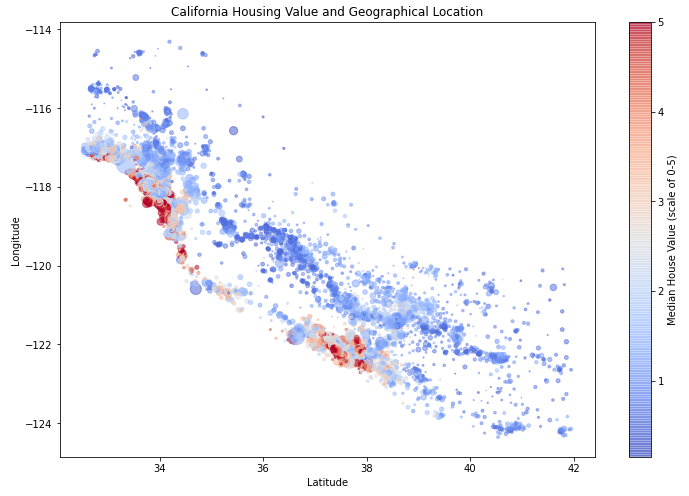
\includegraphics[height=0.8\linewidth]{figures/03_bayesian_linear_regression/california_housing_geoplot.png}
        \subcaption{Geographical data, with red areas indicating high median house price with larger dots indicating higher population.}
    \end{minipage}\hfill
    \begin{minipage}{0.45\textwidth}
        \centering
        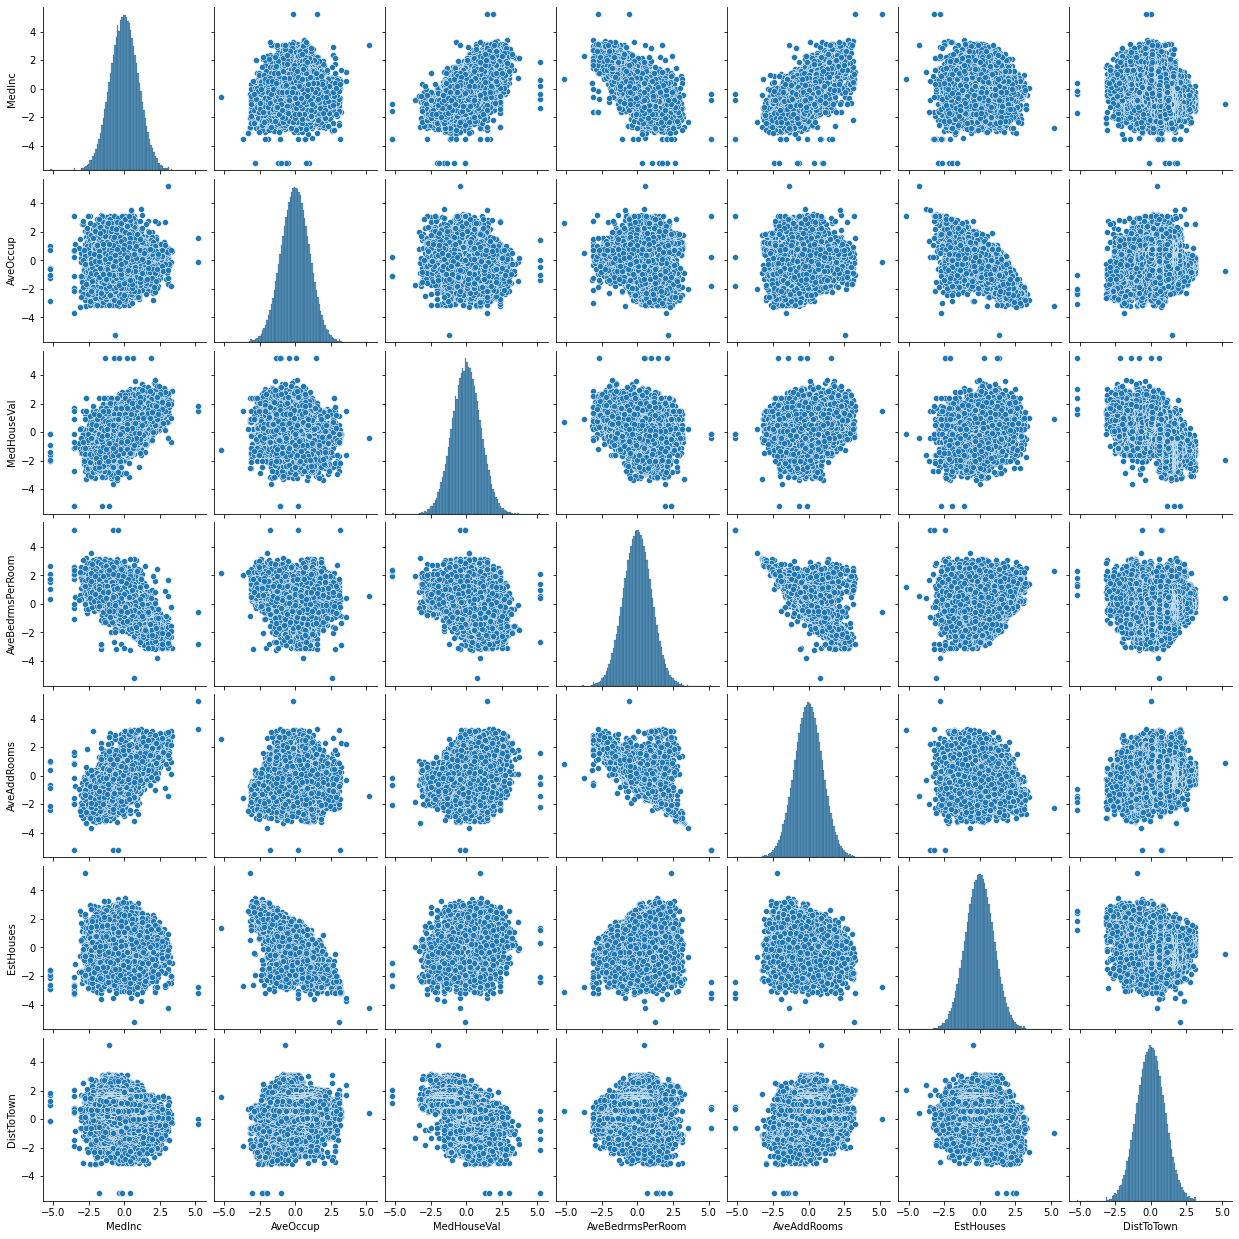
\includegraphics[height=0.8\linewidth]{figures/03_bayesian_linear_regression/california_housing_feature_correlations.png}
        \subcaption{Pair-plot showing pairwise scatter plots for each variable respective histograms on the diagonal.}
    \end{minipage}
\end{figure}

\subsubsection{Bayesian Linear Regression with PyMC3}

Calculating the posterior distributions for the model variables is not possible for continuous variables so Markov Chain Monte Carlo is used to sample from the posterior. With enough samples the distribution of the samples begins to fit that of the posterior distribution; this sampling is done in PyMC3 with the No U-Turn Sampler (NUTS). \\

To create the Bayesian linear regression model with PyMC3 I used the generalised linear model (GLM) module to specify the linear equation to solve in patsy form:

\[ MedHouseVal \sim MedInc + AveOccup + AveBedrmsPerRoom + AveAddRooms + EstHouses + DistToTown \]

This can then be used to specify a GLM with normal priors. 3000 samples are then taken from 8 markov chains with NUTS to approximate the posterior distributions for each of the variables. I have wrapped this as an Sklearn BaseEstimator and RegressorMixin class, where the constructor creates the GLM from a patsy equation and the fit function samples from the Markov chain. 

\subsubsection{Analysing Bayesian Regression Performance}

Bayesian regression produces a distribution of coefficients for each variable so it does not just predict one value, but regression metrics need a single prediction. The mean of the coefficient distribution is the most likely to occur so in analysing performance this is what I shall use. For the Sklearn class the predict function will take the mean of the samples as the coefficients for each variable and make a prediction with that linear model. \\

To measure the performance of different regression models on the data we will use various measures based on the distances of each point to this line. R2 is the coefficient of determination, a measure of distance between the regression line and the real data bound between 0 and 1. A model with a R2 score of 1.0 represents all of the data perfectly. Additionally mean squared error (MSE) takes the mean of the squared distances of all the points to the regression line, with RMSE taking the square root of that as to give worse weighting to models with outlying data. \\

Bayesian linear regression (for mean coefficients) achieve a MSE, RMSE and R2 of $0.37$, $0.61$ and $0.62$ respectively. This is in line with the results of standard linear regression, which makes sense as the priors for each variable are normal and standard linear regression assumes normal features.

\subsubsection{Variable Distributions}

The benefit of Bayesian methods is not necessarily their performance (at their mean), but how they produce a distribution of models rather than a single solution. The Figure \ref{traceplot} shows the KDE plot for each variable and the individual sampled variables for each of the sampling chains. These results show that each of the chains have converged to similar points which helps indicate a strong solution, over trusting a single model to have produced the best result.

\begin{figure}[h]
    \label{traceplot}
    \centering
    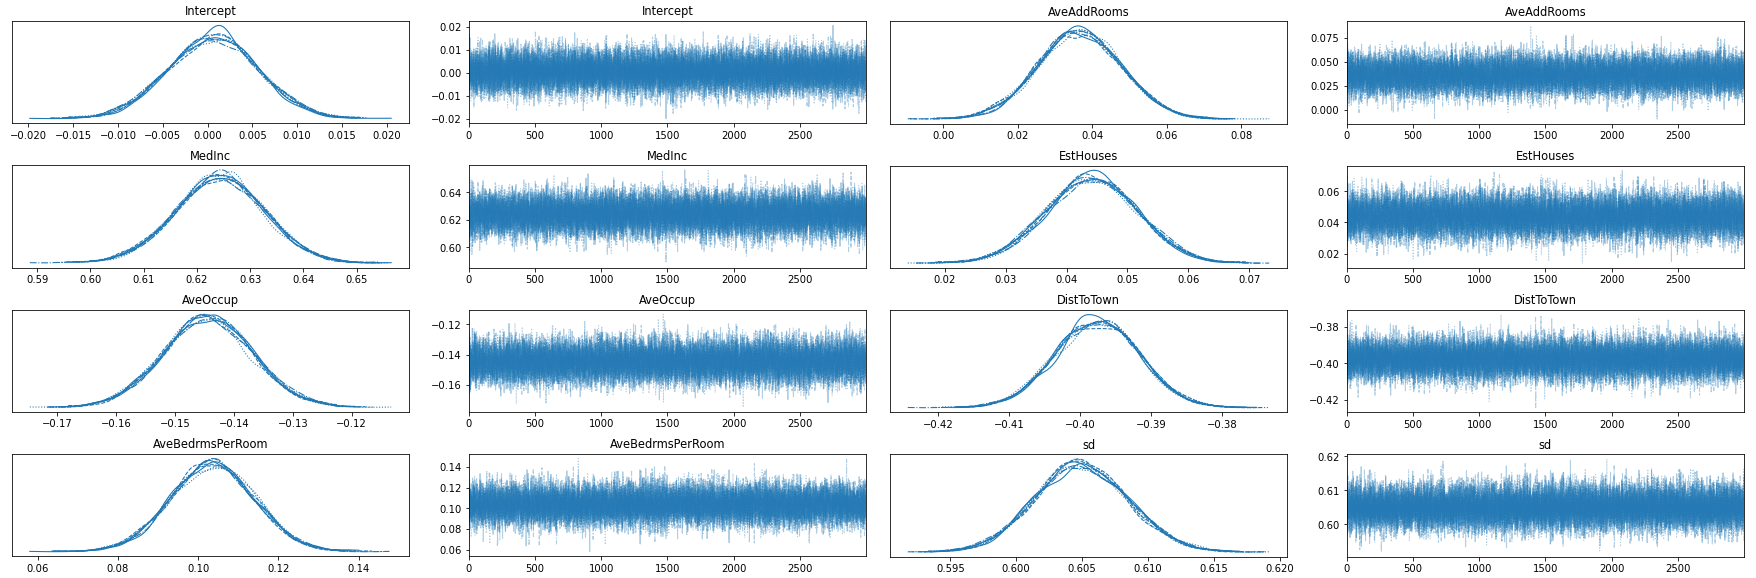
\includegraphics[width=0.95\linewidth]{figures/03_bayesian_linear_regression/bayesian_regression_traceplot.png}
    \caption{KDE plot for each variable (columns 1 and 3) and the individual sampled variables (columns 2 and 4) from Bayesian linear regression.}
\end{figure}

\newpage

%%%%%%%%%%%%%%%%%%%%%%%%%%%%%%%%%%%%%%%%%%%%%%%%%%%%%%%%%%%%%%%%%%%%%%%%%%%%%%%%%%%%%%%%%%%%%%%%%%%%%%%%
%%%%%%%%%%%%%%%%%%%%%%%%%%%%%%%%%%%%%%%%%%%%%%%%%%%%%%%%%%%%%%%%%%%%%%%%%%%%%%%%%%%%%%%%%%%%%%%%%%%%%%%%
%%%%%%%%%%%%%%%%%%%%%%%%%%%%%%%%%%%%%%%%%%%%%%%%%%%%%%%%%%%%%%%%%%%%%%%%%%%%%%%%%%%%%%%%%%%%%%%%%%%%%%%%

\section{Decision Trees and Ensembles}
\label{trees_ensembles}

%%%%%%%%%%%%%%%%%%%%%%%%%%%%%%%%%%%%%%%%%%%%%%%%%%%%%%%%%%%%%%%%%%%%%%%%%%%%%%%%%%%%%%%%%%%%%%%%%%%%%%%%

\subsection{CART Decision Trees}
\label{decision_trees}

Classification and Regression Decision Trees (CART) are a family of supervised models which perform classification or regression using a flow-chart like graph. The tree finds the optimal way to split the training data at each level, an example might be splitting the tree for houses that are less than 10km from LA and those which are not. The combination of these feature splits can result in very complex models being learned.

\subsubsection{Maximum Depth of Decision Trees}
\label{reg_tree_depths}

% If we only look at the training results (red shades) we can see that as max tree depth increases, the performance increases with near-perfect results (R2 of 1 and MSE/RMSE of 0) occurring at depths over 20. This makes sense as the added depth increases the complexity of the model allowing more complex relationships to be learned.

% However looking at the testing results (blue shades) we can see the model is clearly overfitting due to the separation of results between the training and testing sets. If we wish to maximise R2 (on unseen data) it seems a max depth somewhere between 4 and 8 would be ideal, for the testing data this seems to be 6 or 7. Max depths below 4 are underfitting and over 8 there is a lot over overfitting.

% \begin{figure}[h]
%     \centering
%     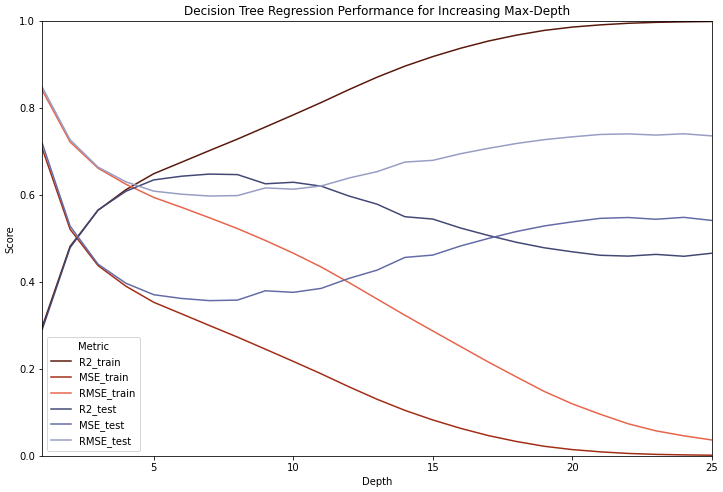
\includegraphics[width=0.6\linewidth]{figures/04_trees_and_ensembles/decision_tree_increasing_depth.png}
%     \subcaption{caption.}
% \end{figure}

\begin{figure}[h]
\floatbox[{\capbeside\thisfloatsetup{capbesideposition={right,top},capbesidewidth=9cm}}]{figure}[\FBwidth]
{\caption{If we only look at the training results (red shades) we can see that as max tree depth increases, the performance increases with near-perfect results (R2 of 1 and MSE/RMSE of 0) occurring at depths over 20. This makes sense as the added depth increases the complexity of the model allowing more complex relationships to be learned. However looking at the testing results (blue shades) we can see the model is clearly overfitting due to the separation of results between the training and testing sets. If we wish to maximise R2 (on unseen data) it seems a max depth somewhere between 4 and 8 would be ideal, for the testing data this seems to be 6 or 7. Max depths below 4 are underfitting and over 8 there is a lot over overfitting..}}
{\fbox{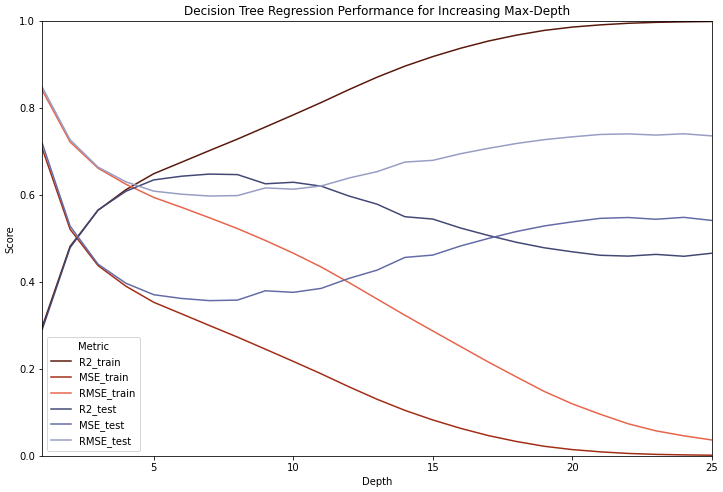
\includegraphics[height=0.65\linewidth]{figures/04_trees_and_ensembles/decision_tree_increasing_depth.png}}}
\label{decision_tree_depths}
\end{figure}

\subsubsection{Hyper-parameter Optimisation}

To find the best decision tree regression model I optimised the maximum depth of the tree and the maximum number of features and the minimum number of samples to split a node and the minimum number of samples for a leaf node. Results from 5-fold cross-validation of the hyper-parameters mentioned show the best model was found when depth is set to $7$, max features are handled automatically by Sklearn, minimum features to split a node is $2$ and the minimum to split a leaf was $9$. Table \ref{04_regression_report} shows the results of the optimal decision tree regressor for the California housing dataset.

\subsubsection{Comparison of Methods}

Table \ref{04_regression_report} shows regression performance of the optimised decision tree regressor and the Bayesian linear regression model for the mean coefficients of the probability distribution. These metrics show the decision tree method has a slight performance advantage, which is likely due to being able to learn non-linear relationships between features where Bayesian linear regression assumes linearity. However this is not the aim of Bayesian regression as we also have a probability distribution of models to draw from which explains a lot more of the data than a single decision tree.

% \begin{wraptable}{r}{5.5cm}
\begin{table}[h]
\begin{tabular}{|l||c|c|c|} 
     \hline
     Method & MSE & RMSE & R2 \\ [0.5ex] 
     \hline
     $Bayesian Regression$ & 0.37 & 0.61 & 0.62 \\ 
     $Decision Tree$       & 0.35 & 0.59 & 0.65  \\ [1ex] 
     \hline
\end{tabular}
\caption{Regression performance of methods on California housing test set.}
\label{04_regression_report}
% \end{wraptable} 
\end{table}

\subsubsection{Decision Tree Visualisation}

The CART algorithm has decided distance to nearest town as being the most deciding feature in the dataset. Median income seems to be the next most important being used all other nodes apart from one with average occupancy. These results align with my analysis of feature correlation after feature engineering, showing that the DistToTown and MedInc are the most correlated with median house value. These findings seem to make sense as housing is more expensive in cities and towns and people with higher income would be expected to have a more expensive house.

\begin{figure}[h]
    \centering
    \fbox{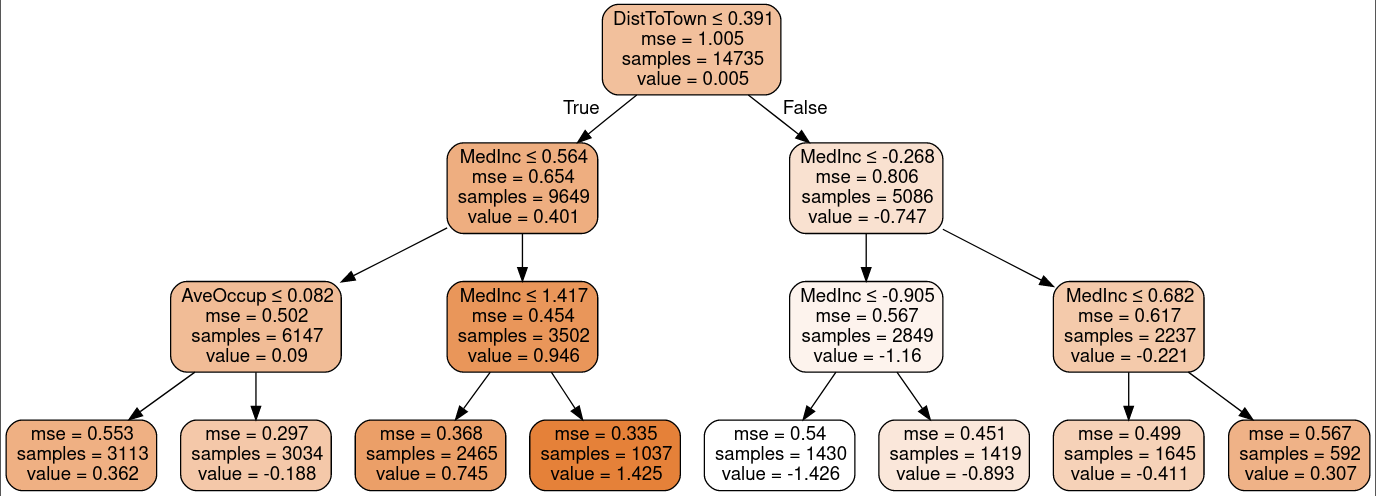
\includegraphics[width=0.7\linewidth]{figures/04_trees_and_ensembles/decision_tree_visualisation.png}}
    \caption{Decision tree trained on California housing dataset with reduced $max\_depth$ of 4 for smaller visualisation.}
\end{figure}

%%%%%%%%%%%%%%%%%%%%%%%%%%%%%%%%%%%%%%%%%%%%%%%%%%%%%%%%%%%%%%%%%%%%%%%%%%%%%%%%%%%%%%%%%%%%%%%%%%%%%%%%

\subsection{Ensembles}
\label{boosting}

\subsubsection{Wisdom of the Crowds}

If you had a large group of people all take an estimate of how many marbles were in a jar you would get a wide range of answers. An expert on marble guessing may be in the top 10\% of closest guesses, but they may still be far off. However if you had access to all these guesses and simply took the median of them all, you would likely be considered better than the experts. This phenomenon is known as the wisdom of the crowd; where the average guess often better than an average guess. \\

Ensemble machine learning methods exploit this, training many models and combining their results into one stronger model. A weak learner is a classifier which just better than guessing. If you created an ensemble of (binary) classifiers each with 51\% accuracy, given enough weak learners, the ensemble model can become a strong learner.

\subsubsection{AdaBoost}

Adaptive boosting (AdaBoost) is an ensemble method which trains a model fit to data, then trains additional models fit to the same dataset but with additional weighting on samples with poor performance. 

\subsubsection{Decision Tree Classification}

As the name CART suggests, decision trees can be also be used for classification tasks. In classification of the MNIST dataset the trees root nodes become the classes (digits) and the nodes of the tree learn to split the samples based on the features (pixel values) in the image. We can then use a decision tree classifier in an AdaBoost ensemble to benefit from the wisdom of the crowds. Optimising the $max\_depth$, $max\_features$, $min\_samples\_split$ and $min\_samples\_leaf$ hyper-parameters of a decision tree classifier with 3-fold cross-validation gives an accuracy of $0.82$; but a default AdaBoost classifier with default decision trees give an accuracy of $0.87$ showing the benefit of this ensemble method over even optimised single models.

\subsubsection{Maximum Depth of Decision Trees in Ensembles}

% We observed section \ref{reg_tree_depths} how regression trees had to be deep enough to learn patterns in the dataset, but also how too much depth can cause overfitting - the same is true for classification trees. 

% \begin{figure}[h]
%     \centering
%     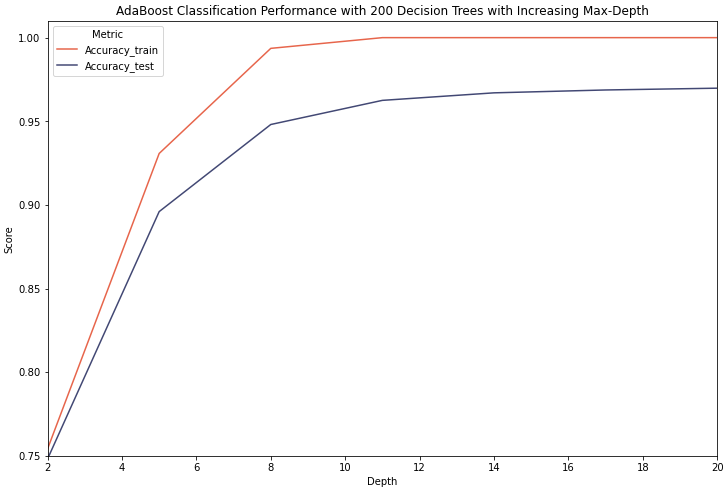
\includegraphics[width=0.6\linewidth]{figures/04_trees_and_ensembles/adaboost_increasing_depth.png}
%     \subcaption{caption.}
% \end{figure}

\begin{figure}[h]
\floatbox[{\capbeside\thisfloatsetup{capbesideposition={right,top},capbesidewidth=9cm}}]{figure}[\FBwidth]
{\caption{We observed section \ref{reg_tree_depths} how regression trees had to be deep enough to learn patterns in the dataset- the same is true for classification trees. However from the results observed here it seems that overfitting is not as much of an issue. This is likely due to having a large number of trees; each individual tree is not guaranteed to produce the same solution with some out performing others. It is common to train many decision trees and select the best, but with an ensemble method there is no need as they will combine their knowledge to produce a more general solution, hence less overfitting.}}
{\fbox{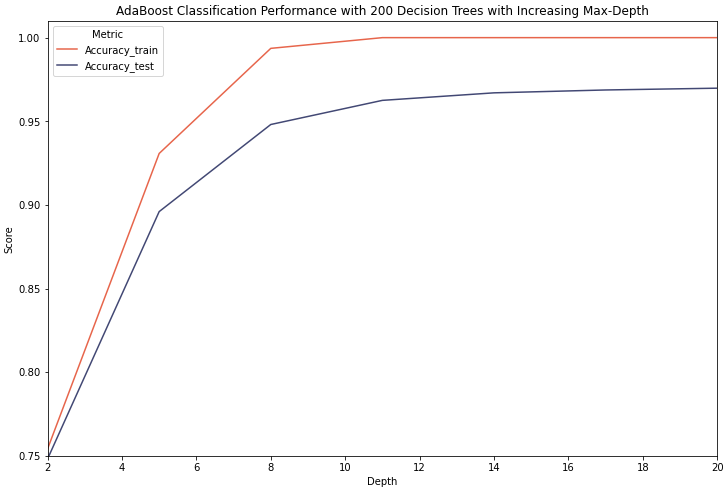
\includegraphics[height=0.65\linewidth]{figures/04_trees_and_ensembles/adaboost_increasing_depth.png}}}
\label{adaboost_depths}
\end{figure}

\subsubsection{Hyper-parameter Optimisation}

The two main hyper-parameters to optimise for with AdaBoost are the maximum number of decision trees in the ensemble (if perfect accuracy is achieved before the max trees are added then boosting stops) and the learning rate which determines the weighting of new models added to the ensemble. My testing found that a learning rate of 1 with 200 decision trees of maximum depth of 16 was optimal, reaching an accuracy of $0.96$.

\subsubsection{Comparison of Methods}

When comparing classification models it is often a good idea to analyse the relationship between true positive, true negative, false positive and false negative classifications rather than outright accuracy as it can give insight into their strengths and weaknesses. Recall measures the proportion of positive detections out of all the positive, precision measures the proportion of correct detections from all of the detections and $F_1$-score is the harmonic mean of precision and recall, meaning a detector with a high $F_1$ will have both high precision and recall which should result in accurate classifications with few mistakes. \\

Table \ref{04_classification_report} shows the final classification performances of the methods discussed in sections \ref{classifiers} and \ref{trees_ensembles}. It is clear that the CNN model has outperformed the others, but this is no be expected as this method is quite image specific. The AdaBoost method has performed on par with the neural network, whilst being much less complex in design and only just beat out by the RBF-kernel SVM. The single decision tree is the poorest method with a $F_1$ of $0.82$, whilst the AdaBoost ensemble scored $0.97$ showing its strength and of ensembles in general.

% \begin{wraptable}{r}{5.5cm}
\begin{table}[h]
\begin{tabular}{|l||c|c|c|} 
     \hline
     Method & Precision & Recall & $F_1$ \\ [0.5ex] 
     \hline
     $ANN$           & 0.97 & 0.97 & 0.97 \\ 
     $CNN$           & 0.99 & 0.99 & 0.99 \\ 
     $RBFSVM$        & 0.98 & 0.98 & 0.98 \\ 
     $Decision Tree$ & 0.82 & 0.82 & 0.82 \\ 
     $AdaBoost$      & 0.97 & 0.97 & 0.97 \\ [1ex] 
     \hline
\end{tabular}
\caption{Classification performance of methods on MNIST test set.}
\label{04_classification_report}
% \end{wraptable} 
\end{table}

%%%%%%%%%%%%%%%%%%%%%%%%%%%%%%%%%%%%%%%%%%%%%%%%%%%%%%%%%%%%%%%%%%%%%%%%%%%%%%%%%%%%%%%%%%%%%%%%%%%%%%%%

%%%%%%%%%%%%%%%%%%%%%%%%%%%%%%%%%%%%%%%%%%%%%%%%%%%%%%%%%%%%%%%%%%%%%%%%%%%%%%%%%%%%%%%%%%%%%%%%%%%%%%%%
%%%%%%%%%%%%%%%%%%%%%%%%%%%%%%%%%%%%%%%%%%%%%%%%%%%%%%%%%%%%%%%%%%%%%%%%%%%%%%%%%%%%%%%%%%%%%%%%%%%%%%%%
%%%%%%%%%%%%%%%%%%%%%%%%%%%%%%%%%%%%%%%%%%%%%%%%%%%%%%%%%%%%%%%%%%%%%%%%%%%%%%%%%%%%%%%%%%%%%%%%%%%%%%%%

% include your own bib file like this:
% \bibliographystyle{coling}
% \bibliography{coling2020}

\end{document}
